\section{Experiments}
\label{sec:experiments}

% Number sources (all FLUX.1-dev, DrawBench-200, eval2 paired bootstrap, 10k resamples, seed 0):
%   research_v2/runs/drawbench_eval/eval_two_budgets_vs_seacache.txt, eval_sweep_vs_seacache.txt,
%   eval_sweep_vs_kalsea.txt, eval_final.txt, eval_dct_pcgs.txt, eval_pairs2.txt; linear extrapolation =
%   runs/drawbench/linext_<d> (generic first-order extrapolation, metrics_sweep/main.json), paired
%   bootstrap recomputed with the eval2 procedure. Correction sizes: plugin_stats (dx_rel, gap_len) in the stats files of
%   research_v2/runs/drawbench/kalsea_dct_pcgs_<d>.

\subsection{Setup}
\label{sec:setup}

\paragraph{Models and protocol.}
We follow the protocol of \seacache~\cite{chung2026seacache}. For text-to-image generation we use
\flux~\cite{blackforestlabs2024flux} at $1024{\times}1024$ with 50 Euler steps of its default flow-matching schedule,
embedded guidance 3.5, and the 200 DrawBench prompts~\cite{saharia2022imagen}; the seed of each image is its prompt
index and is shared by all methods. For text-to-video generation we use HunyuanVideo~\cite{kong2024hunyuanvideo} at
$480{\times}640$ with 65 frames and Wan2.1-T2V-1.3B~\cite{wan2025wan} at $832{\times}480$ with 81 frames, both with 50
steps, on the 944 unique VBench prompts~\cite{huang2024vbench}. \TODO{Video seeds.} Each accelerated sample is compared
with the output of the uncached 50-step sampler for the same prompt and seed.

\paragraph{Budgets and baselines.}
All caches use the official \sea gate, and the budget is set by its threshold $\delta$. We report the mean number of
block-stack evaluations per image (\nfe, out of 50), counted by hooks on every block. Since the gate is closed-loop and
\pcgs refreshes its reference, different fillers can produce slightly different schedules; we only compare at matched
\nfe. On \flux, $\delta=0.3$ and $0.6$ give 20.8 and 13.0 \nfe, and at $\delta=0.6$ our run of \seacache reproduces its
published PSNR (21.26 vs.\ 21.33\,dB~\cite{chung2026seacache}). At these two thresholds \seacache, \kalsea and \ours
computed exactly the same steps for 188 and 182 of the 200 prompts, and the per-prompt \nfe never differs by more than
one, so the comparison isolates what is written on skipped steps. Behind the same gate we compare four fillers: reuse of
the last residual (\seacache), linear extrapolation of the residual from the last two computed steps (the first-order
finite-difference forecast of TaylorSeer~\cite{liu2025taylorseer}), the Kalman forecast (\kalsea), and the Kalman
forecast with \pcgs (\ours). \TODO{Rows for TeaCache, TaylorSeer, $\Delta$-DiT and ToCa at matched budgets, if run.}

\paragraph{Metrics.}
We report PSNR on 8-bit RGB, SSIM~\cite{wang2004ssim} (scikit-image, $7{\times}7$ window) and LPIPS with AlexNet
features~\cite{zhang2018lpips}, each against the 50-step reference and averaged over prompts. For differences between
methods we report paired bootstrap 95\% confidence intervals over prompts (10{,}000 resamples, percentile intervals)
and the fraction of prompts on which a method is better. \TODO{TFLOPs (counted as in \seacache) and latency, measured
for all methods under identical conditions; until then the tables show \nodata.}

\paragraph{Development and test prompts.}
All design decisions (the smoother, the re-integration and continuation rules, $\tau$ and $R$) were made on a
development set of 64 COCO captions~\cite{lin2014coco}, and the forecaster was calibrated on 16 other COCO captions.
DrawBench was only used to score finished configurations and is thus a held-out test set. Development-set results are
reported in the supplement.

\paragraph{Implementation.}
\ours replaces the forward pass of the transformer in diffusers; the scheduler is unchanged, and the re-integration
\eqref{eq:reint} reproduces its arithmetic. All runs use bf16 on NVIDIA B200 GPUs. For video we use the per-element
filter, since the DCT bands are defined on 2D token grids. \TODO{Video implementation details (calibration, UniPC
replay for Wan2.1).}

\maybeinput{tables/tab_flux_main}

\subsection{Comparison at matched \nfe}
\label{sec:main-results}

\cref{tab:flux-main} compares the fillers at the two budgets of the protocol. At 20.8 \nfe, \ours improves over
\seacache by 2.73\,dB PSNR (95\% CI [2.34, 3.12]; better on 88\% of the prompts), 0.031 SSIM [0.027, 0.036] and
0.033 LPIPS [0.029, 0.037]. At 13 \nfe the gains are 1.27\,dB [1.02, 1.52] (79\% of the prompts), 0.042 SSIM
[0.035, 0.048] and 0.060 LPIPS [0.052, 0.068]. Forecasting explains part of this improvement, as both forecasters
improve over reuse: linear extrapolation reaches 28.51 and 21.80\,dB and \kalsea 28.79 and 21.91\,dB at the two budgets.
\pcgs adds 0.83\,dB [0.63, 1.02] at 20.8 \nfe and 0.61\,dB [0.48, 0.76] at 13 \nfe on top of \kalsea, with better PSNR
on 81\% and 78\% of the prompts, and \ours exceeds linear extrapolation by 1.11\,dB [0.89, 1.34] and 0.73\,dB
[0.54, 0.92]. The median per-prompt gain of \pcgs over \kalsea is 0.60 and 0.44\,dB; on the remaining 19\% and 22\% of
the prompts it lowers PSNR, by at most 3.6 and 2.3\,dB.
% Linear extrapolation is not in tab_flux_main (generated by figures/src/make_tables.py); NFE 20.84 / 13.00, SSIM
% 0.925 / 0.827, LPIPS 0.061 / 0.171. Suggest adding it as a row "Lin. extrapolation" (generic baseline).

\begin{figure*}[t]
  \centering
  \maybegraphics[width=\textwidth]{figures/fig_tradeoff.pdf}
  \IfFileExists{figures/fig_tradeoff_caption.tex}{% Auto-generated by figures/src/make_captions.py (numbers from figures/src/data). Usage:
% \begin{figure*}[t]\centering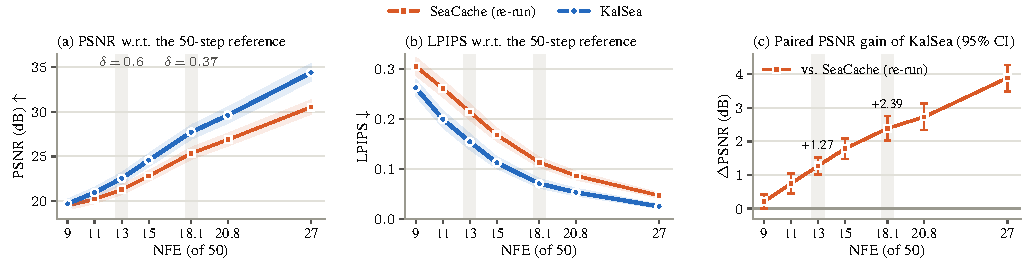
\includegraphics[width=\textwidth]{figures/fig_tradeoff.pdf}% Auto-generated by figures/src/make_captions.py (numbers from figures/src/data). Usage:
% \begin{figure*}[t]\centering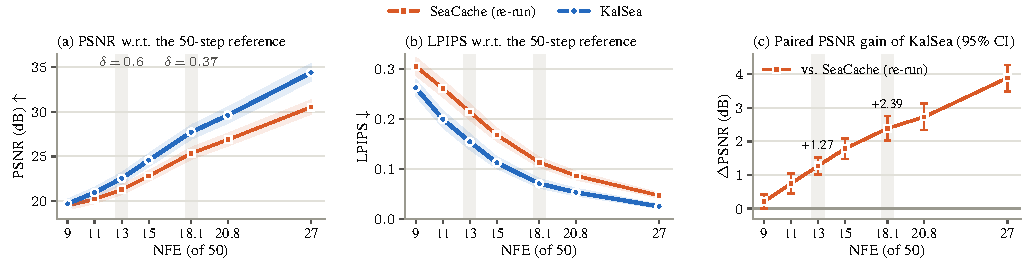
\includegraphics[width=\textwidth]{figures/fig_tradeoff.pdf}% Auto-generated by figures/src/make_captions.py (numbers from figures/src/data). Usage:
% \begin{figure*}[t]\centering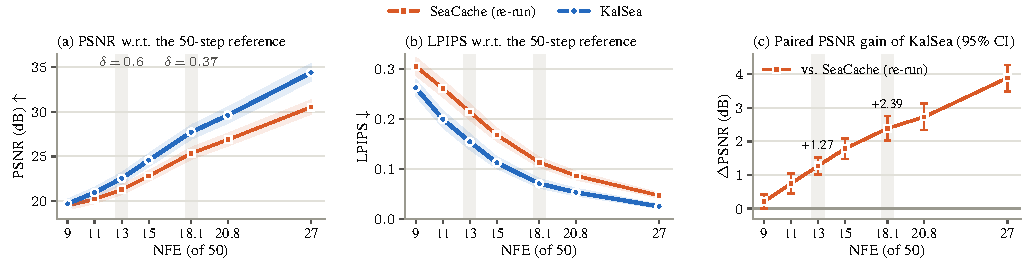
\includegraphics[width=\textwidth]{figures/fig_tradeoff.pdf}\input{figures/fig_tradeoff_caption}\end{figure*}   (one-column variant: figures/fig_tradeoff_1col.pdf, width=\columnwidth, same caption)
\caption{\textbf{Quality--compute trade-off on \flux} (DrawBench, 200 held-out prompts). \textbf{(a)}~PSNR and \textbf{(b)}~LPIPS with respect to the 50-step reference vs.\ the mean number of transformer evaluations per image (\nfe). The budget is set by the \sea-gate threshold $\delta \in \{0.2, 0.3, 0.37, 0.5, 0.6, 0.8, 1.0\}$, shared by all methods; gray bands mark the two budgets of \cref{tab:flux-main} ($\delta = 0.3$, $0.6$). Lines: means over prompts; shaded: 95\% bootstrap CIs. \textbf{(c)}~Paired per-prompt PSNR gain of \ours over \seacache and over \kalsea (mean, 95\% bootstrap CI). The gain over \seacache grows with the budget, from +0.21\,dB [$-$0.005, +0.42] at 9 \nfe (not significant; LPIPS still improves by 0.043 [0.033, 0.053]) to +3.89\,dB [+3.49, +4.28] at 27 \nfe; the gain over \kalsea (gap smoothing alone) is positive at every budget. \seacache: \sea gate with residual reuse; \kalsea: \sea gate with Kalman residual forecasting; \ours: \kalsea with predictor-corrector gap smoothing.}
\label{fig:tradeoff}
\end{figure*}   (one-column variant: figures/fig_tradeoff_1col.pdf, width=\columnwidth, same caption)
\caption{\textbf{Quality--compute trade-off on \flux} (DrawBench, 200 held-out prompts). \textbf{(a)}~PSNR and \textbf{(b)}~LPIPS with respect to the 50-step reference vs.\ the mean number of transformer evaluations per image (\nfe). The budget is set by the \sea-gate threshold $\delta \in \{0.2, 0.3, 0.37, 0.5, 0.6, 0.8, 1.0\}$, shared by all methods; gray bands mark the two budgets of \cref{tab:flux-main} ($\delta = 0.3$, $0.6$). Lines: means over prompts; shaded: 95\% bootstrap CIs. \textbf{(c)}~Paired per-prompt PSNR gain of \ours over \seacache and over \kalsea (mean, 95\% bootstrap CI). The gain over \seacache grows with the budget, from +0.21\,dB [$-$0.005, +0.42] at 9 \nfe (not significant; LPIPS still improves by 0.043 [0.033, 0.053]) to +3.89\,dB [+3.49, +4.28] at 27 \nfe; the gain over \kalsea (gap smoothing alone) is positive at every budget. \seacache: \sea gate with residual reuse; \kalsea: \sea gate with Kalman residual forecasting; \ours: \kalsea with predictor-corrector gap smoothing.}
\label{fig:tradeoff}
\end{figure*}   (one-column variant: figures/fig_tradeoff_1col.pdf, width=\columnwidth, same caption)
\caption{\textbf{Quality--compute trade-off on \flux} (DrawBench, 200 held-out prompts). \textbf{(a)}~PSNR and \textbf{(b)}~LPIPS with respect to the 50-step reference vs.\ the mean number of transformer evaluations per image (\nfe). The budget is set by the \sea-gate threshold $\delta \in \{0.2, 0.3, 0.37, 0.5, 0.6, 0.8, 1.0\}$, shared by all methods; gray bands mark the two budgets of \cref{tab:flux-main} ($\delta = 0.3$, $0.6$). Lines: means over prompts; shaded: 95\% bootstrap CIs. \textbf{(c)}~Paired per-prompt PSNR gain of \ours over \seacache and over \kalsea (mean, 95\% bootstrap CI). The gain over \seacache grows with the budget, from +0.21\,dB [$-$0.005, +0.42] at 9 \nfe (not significant; LPIPS still improves by 0.043 [0.033, 0.053]) to +3.89\,dB [+3.49, +4.28] at 27 \nfe; the gain over \kalsea (gap smoothing alone) is positive at every budget. \seacache: \sea gate with residual reuse; \kalsea: \sea gate with Kalman residual forecasting; \ours: \kalsea with predictor-corrector gap smoothing.}
\label{fig:tradeoff}
}{%
  \caption{\textbf{Fidelity versus compute on \flux} (DrawBench, 200 held-out prompts). The \sea-gate threshold
    $\delta\in\{1.0, 0.8, 0.6, 0.5, 0.37, 0.3, 0.2\}$ sets the budget (9 to 27 of 50 transformer evaluations); all
    methods share the gate and are compared at matched \nfe. \textbf{(a)}~PSNR and \textbf{(b)}~LPIPS with respect to
    the 50-step sampler; shaded bands are 95\% bootstrap confidence intervals of the mean. \textbf{(c)}~Paired PSNR gain
    of \ours over \seacache and over \kalsea, with 95\% confidence intervals. Gray columns mark the two budgets of
    \cref{tab:flux-main}; all numbers are listed in the supplement.}
  \label{fig:tradeoff}}
\end{figure*}

\paragraph{Budget sweep.}
\cref{fig:tradeoff} varies $\delta$ from 0.2 to 1.0 (27 to 9 \nfe). \ours attains the highest PSNR and the lowest LPIPS
at every budget. Its PSNR gain over \seacache grows with the budget, from 0.74\,dB [0.46, 1.04] at 11 \nfe to 3.89\,dB
[3.49, 4.28] at 27 \nfe; at 9 \nfe the PSNR gain is not significant (0.21\,dB [$-$0.005, 0.42]), whereas LPIPS still
improves by 0.043 [0.033, 0.053]. The predictor alone behaves as the open-loop argument of \cref{sec:intro} predicts:
the gain of \kalsea over reuse shrinks from 2.37\,dB at 27 \nfe to 0.11\,dB [$-$0.14, 0.34] at 11 and $-$0.10\,dB
[$-$0.31, 0.10] at 9 \nfe, and linear extrapolation even falls below reuse at 11 and 9 \nfe ($-$0.58 and $-$0.77\,dB),
because forecast errors accumulate over the long gaps of small budgets. \pcgs improves on \kalsea at every budget, by
0.31\,dB [0.24, 0.39] at 9 \nfe and up to 1.52\,dB [1.30, 1.75] at 27 \nfe.

\paragraph{Size of the correction.}
The relative latent correction $\|\lat'_b-\lat_b\|/\|\lat_b\|$ grows with the length of the gap. At 13 \nfe it
averages 0.7\% after single skipped steps and 4.1\% after the seven-step gaps, which contain a third of all skipped
steps (2.0\% over all gaps); at 20.8 \nfe, where most skipped steps lie in three-step gaps, it averages 0.7\%.

\begin{figure*}[t]
  \centering
  \maybegraphics[width=\textwidth]{figures/fig_qualitative.pdf}
  \IfFileExists{figures/fig_qualitative_caption.tex}{% Auto-generated by figures/src/make_captions.py (numbers from figures/src/data). Usage:
% \begin{figure*}[t]\centering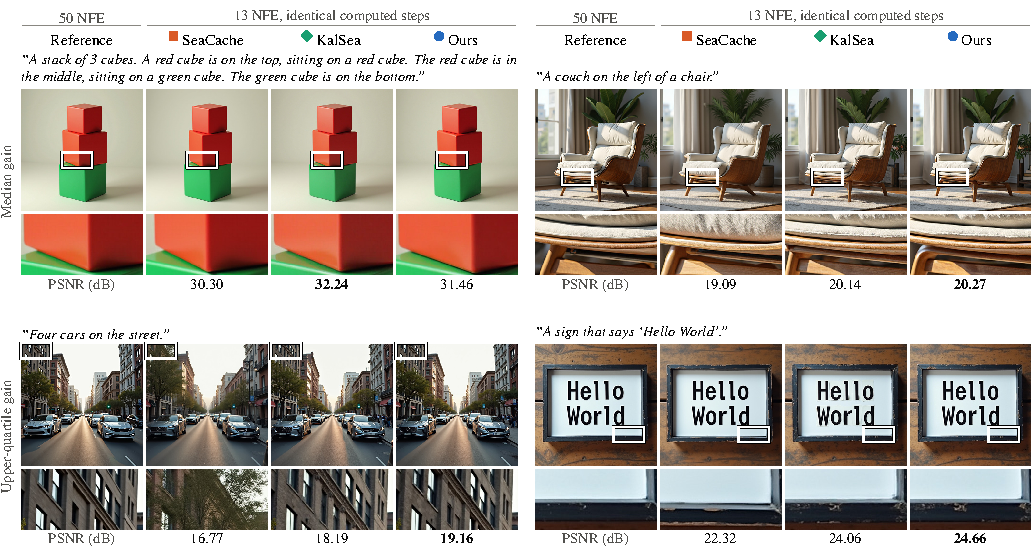
\includegraphics[width=\textwidth]{figures/fig_qualitative.pdf}% Auto-generated by figures/src/make_captions.py (numbers from figures/src/data). Usage:
% \begin{figure*}[t]\centering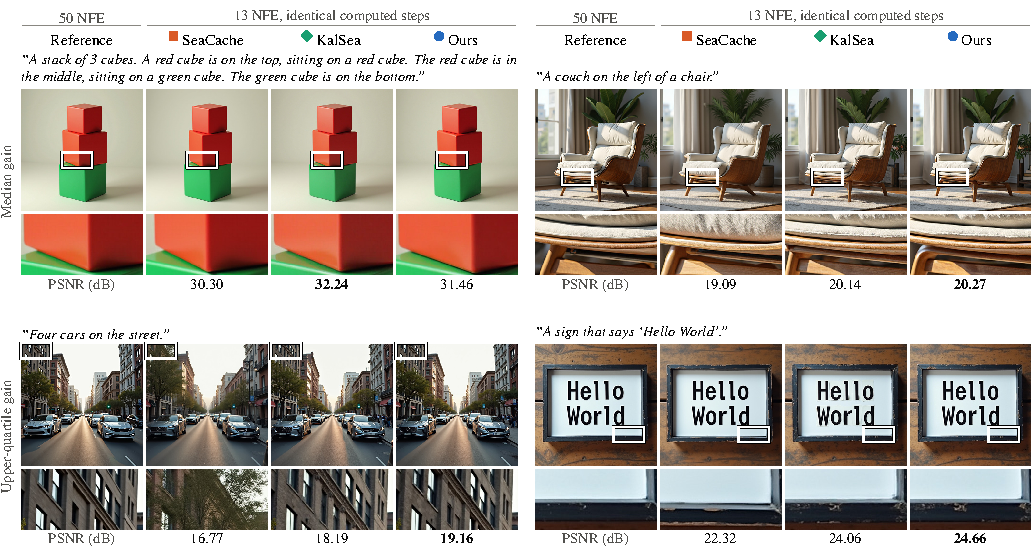
\includegraphics[width=\textwidth]{figures/fig_qualitative.pdf}% Auto-generated by figures/src/make_captions.py (numbers from figures/src/data). Usage:
% \begin{figure*}[t]\centering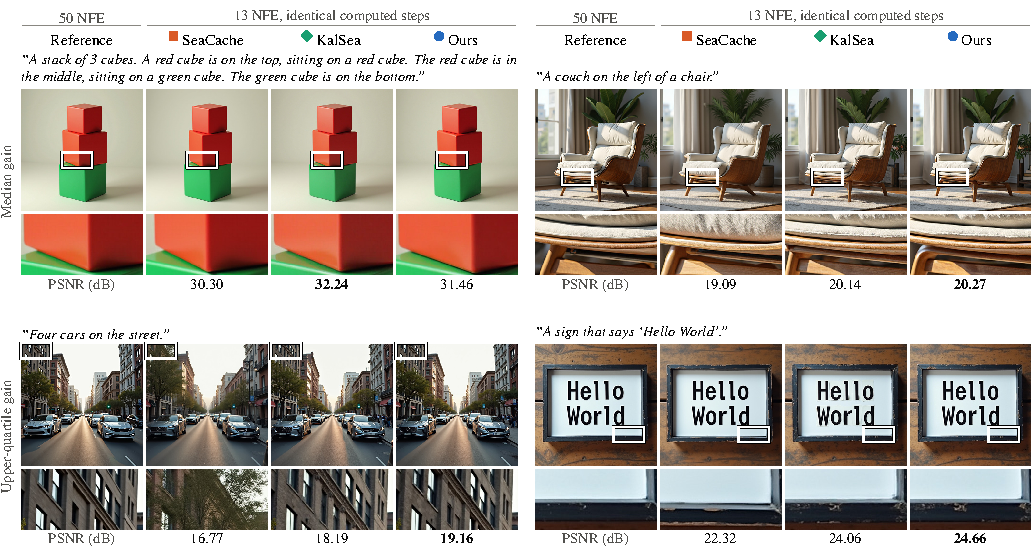
\includegraphics[width=\textwidth]{figures/fig_qualitative.pdf}\input{figures/fig_qualitative_caption}\end{figure*}
\caption{\textbf{Qualitative comparison at 13 \nfe} (\flux, DrawBench, $\delta = 0.6$, $3.8\times$ fewer transformer evaluations than the 50-step reference). The prompts are selected by a fixed rule, not by hand: among the 188 of 200 prompts on which \seacache and \ours computed the identical set of steps, we compute the per-prompt PSNR gain of \ours over \seacache and show the two prompts whose gain is closest to the median (+1.19\,dB; top row) and the two closest to the upper quartile (+2.40\,dB; bottom row). Below each image, a fixed $256\times128$-pixel crop (of $1024\times1024$) is magnified; it is placed where the two accelerated samples differ most (largest mean absolute difference), without looking at the reference. Numbers: PSNR (dB) with respect to the reference, best in bold. Examples near the lower quartile and at the $\approx$21-\nfe budget are in the supplementary material.}
\label{fig:qualitative}
\end{figure*}
\caption{\textbf{Qualitative comparison at 13 \nfe} (\flux, DrawBench, $\delta = 0.6$, $3.8\times$ fewer transformer evaluations than the 50-step reference). The prompts are selected by a fixed rule, not by hand: among the 188 of 200 prompts on which \seacache and \ours computed the identical set of steps, we compute the per-prompt PSNR gain of \ours over \seacache and show the two prompts whose gain is closest to the median (+1.19\,dB; top row) and the two closest to the upper quartile (+2.40\,dB; bottom row). Below each image, a fixed $256\times128$-pixel crop (of $1024\times1024$) is magnified; it is placed where the two accelerated samples differ most (largest mean absolute difference), without looking at the reference. Numbers: PSNR (dB) with respect to the reference, best in bold. Examples near the lower quartile and at the $\approx$21-\nfe budget are in the supplementary material.}
\label{fig:qualitative}
\end{figure*}
\caption{\textbf{Qualitative comparison at 13 \nfe} (\flux, DrawBench, $\delta = 0.6$, $3.8\times$ fewer transformer evaluations than the 50-step reference). The prompts are selected by a fixed rule, not by hand: among the 188 of 200 prompts on which \seacache and \ours computed the identical set of steps, we compute the per-prompt PSNR gain of \ours over \seacache and show the two prompts whose gain is closest to the median (+1.19\,dB; top row) and the two closest to the upper quartile (+2.40\,dB; bottom row). Below each image, a fixed $256\times128$-pixel crop (of $1024\times1024$) is magnified; it is placed where the two accelerated samples differ most (largest mean absolute difference), without looking at the reference. Numbers: PSNR (dB) with respect to the reference, best in bold. Examples near the lower quartile and at the $\approx$21-\nfe budget are in the supplementary material.}
\label{fig:qualitative}
}{%
  \caption{\textbf{Qualitative comparison on \flux at 13 \nfe} (held-out DrawBench prompts). For these prompts the
    three caches computed the same steps. Prompts are chosen by a fixed rule: among the prompts with identical
    schedules, those whose PSNR gain of \ours over \seacache is closest to the median (top) and to the upper quartile
    (bottom). Zoom windows are placed where the three cached images differ most from each other, without using the
    reference. Numbers: PSNR with respect to the 50-step sampler.}
  \label{fig:qualitative}}
\end{figure*}

\paragraph{Qualitative results.}
\cref{fig:qualitative} shows prompts selected by a fixed rule rather than by hand. With the same computed steps, reuse
blurs or alters high-frequency structure such as facades and upholstery, the Kalman forecast recovers part of it, and
\pcgs brings the details closer to the reference. The improvement is not uniform: on some prompts the predictor alone
is already as close to the reference as \ours. \TODO{Sync with the final figure; more examples at 13 and 20.8 \nfe in
the supplement.}

\subsection{Video generation}
\label{sec:video}

\maybeinput{tables/tab_video_main}

We apply \ours with the per-element filter to HunyuanVideo and Wan2.1-1.3B at the two thresholds of \seacache
(HunyuanVideo: $\delta=0.19$ and 0.35; Wan2.1: $\delta=0.2$ and 0.35). HunyuanVideo samples with Euler steps and a
single guidance-distilled branch, so \pcgs applies exactly as in \cref{sec:pcgs}; Wan2.1 uses UniPC with
classifier-free guidance and requires the solver replay described there. \cref{tab:video-main} reports the results.
\TODO{Results and discussion; VBench scores in the supplement.}

\subsection{Ablations}
\label{sec:ablations}

\maybeinput{tables/tab_ablation_2x2}

\paragraph{Forecaster parametrization.}
\cref{tab:ablation-2x2} crosses the two parametrizations of the predictor with \pcgs. \pcgs improves both by similar
amounts: by 0.78\,dB [0.60, 0.97] and 0.61\,dB [0.48, 0.75] with DCT bands, and by 0.83\,dB [0.66, 1.01] and 0.58\,dB
[0.44, 0.73] per element, at 18.1 and 13 \nfe. With \pcgs, the two parametrizations differ by 0.02\,dB [$-$0.09, 0.15]
and 0.01\,dB [$-$0.13, 0.15]. Unlike for forecasting the model output~\cite{rajabi2026speckcast}, the frequency
decomposition is unnecessary for the residual, and the simpler per-element filter suffices; we use it for video.
% The DCT rows without PCGS in tab_ablation_2x2 are the same-harness rerun of KalSea (kalsea_main_<d>), which differs
% from the KalSea run in tab_flux_main / fig_tradeoff (speckcast_<d>) by +0.03 / +0.00 dB.

\maybeinput{tables/tab_ablation_main}

\paragraph{Anatomy of the corrector.}
\cref{tab:ablation} isolates the parts of \pcgs on DrawBench at 20.8 and 13 \nfe. \TODO{Numbers from the generated
ablation table once the runs are scored; report each row as a paired difference to \ours.}
% Table: tables/tab_ablation_main.tex, generated by research_v2/ablations/make_tables.py with \label{tab:ablation}.
The rows compare: correcting only the filter state, without re-integrating
the latent (\tbd); re-integration with a linear interpolation from $\res_a$ to $\res_b$ that ignores the forecast
(\tbd), with the forecast plus a linearly weighted innovation (\tbd), with a quadratic interpolation through the last
three computed residuals (\tbd), and with the RTS gains (\ours); a batched re-integration that reuses the stored inputs
$\hin_i$ instead of re-embedding the corrected latents (\tbd); and \pcgs without the gate refresh (\tbd). On the
development set, the exact re-integration was better than the batched one by 0.36\,dB at 18 \nfe (0.10\,dB at 13 \nfe,
not significant), the linear interpolation performed similarly to the RTS gains (difference $-$0.13 and $+$0.07\,dB,
both intervals include zero), and the gate refresh had no measurable effect (supplement).
% Development-set numbers: research_v2/ablations/ABLATIONS_devset.md (COCO-64, n = 62-64, per-element forecaster).

\paragraph{Other fillers and forecaster settings.}
The correction is not tied to the Kalman forecaster. With reuse, the corresponding smoother interpolates linearly
between $\res_a$ and $\res_b$; on the development set this improves reuse by 1.31\,dB [1.00, 1.59] and 0.77\,dB
[0.57, 0.97] at 18 and 13 \nfe. \TODO{DrawBench rows: reuse + \pcgs and linear extrapolation + \pcgs (\tbd).} We also
test the trend damping $\tau=0.1$ used by SpecKCast (\tbd). With a calibration-free per-element filter, \pcgs still
adds 0.83 and 0.51\,dB on the development set. Forecasting a quantity of the sampler instead of the residual (the
clean-image, noise or velocity prediction reconstructed from the current latent) was not better on the development
set (supplement).

\paragraph{Noise floor.}
The band statistics of the filter are accumulated with atomic GPU additions, so two runs of the same configuration are
not bitwise identical. Two runs of \kalsea differ by 0.03\,dB [$-$0.003, 0.067] at 18.1 \nfe and by 0.002\,dB
[$-$0.008, 0.011] at 13 \nfe in mean PSNR; we make no claims about differences below 0.1\,dB.
